\documentclass[conference]{IEEEtran}

%+++++++++++++++++++++++++++++++++++++++++++++++++++
\usepackage[pdftex]{graphicx}
\usepackage{amsmath}
\usepackage{eqparbox}
%+++++++++++++++++++++++++++++++++++++++++++++++++++


\hyphenation{op-tical net-works semi-conduc-tor IEEEtran}
\begin{document}

%+++++++++++++++++++++++++++++++++++++++++++++++++++
\title{\LARGE SUNFLOWER: A Trust Execution Environment on RISCV \\Based on Tagged Memory}
\author{\authorblockN{Xu Jinyan 316010**** Duan Yuxuan 316010**** Lin Yizhu 316010****} }
% \authorblockA{\authorrefmark{1}Leave Affiliation List blank for your Summary (initial) submission}}
%+++++++++++++++++++++++++++++++++++++++++++++++++++

\maketitle


% ================
% # Abstract     #
% ================

\begin{abstract}
This is a report for the class: Network Security Theory and Practice, our project is aimed to build a execution environment in RISC-V using tagged memory technology. RISC-V is an open and extensible instruction set architecture designed by UC Berkly, because of its low overhead, it's very suitable for using in the embedded devices and internet of things. As with the various system vulnerabilities recently exposed, operating systems are no longer fully trusted. More and more people choose to using the hardware security method, like Trust Zone(ARM), SGX(Intel). However, there are still no officically supported safety standards for RISC-V.

Here, we design a tagged memory hardware security architecture, inspired by the paper[1]. Tagged memory has been proposed as a fine-grained security mechanism to support protection of data flow, pointers or capabilities for a long time, but none of the existing schemes provide efficient and flexible at the same time, it is still a open problem. We using tag-aware instruction and a simple kernel to achieve a fine-grained isolation. We also provide a series of tools for easy to use, a gcc and objdump supported tag-aware instructions. And we finish our logical design in Spike, a RISC-V simulator.
\end{abstract}

\begin{keywords}
RISC-V, tagged memory, tag-aware instruction set architecture.
\end{keywords}


% ========================
% # I. Introduction      #
% ========================

\section{Introduction}
IoT devices are rapidly entering everyday life. However, these devices have a great risk to be attacked since the code of these devices are complex thus potential to have bugs. To ensure the security of the applications running on these devices even when the devices are compromised, a kind of skill called Trusted Execution Environment(TEE) can be of great help. The main idea of TEE is to use isolated execution to protect trusted applications from compromised operating systems or other untrusted software on the same device.

Recent years have witnessed many implementations of TEE on different systems. ARM TrustZone and Intel SGX are two widely applied TEE architectures. ARM TrustZone divides the computer resources into a secure and non-secure world on hardware level.\cite{TrustZone} The secure world can access all system resources while the non-secure world can only access data in the non-secure world or call secure applications through designed secure entry points. With TrustZone architecture, if sensitive data and code are hidden in the secure world, they cannot be accessed by untrusted applications or system. However, TrustZone needs a secure kernel to manage the secure world, providing secure system services, thus enlarge the trusted computing base(TCB), which increases the risk. Intel SGX uses an isolated container called enclave which hold sensitive part of applications.\cite{SGX} Unlike TrustZone, SGX does not need any privileged supervisor like a trusted kernel, thus reduces TCB. But SGX needs complex instructions to manage enclaves.

Resource-constrained devices like IoT devices often have little memory, thus needs fine-grained memory management. The isolation boundary the existing implementations of TEE provides are not fine-grained enough for small IoT devices to apply.\cite{TIMBERV} Inspired by the work in \cite{TIMBERV}, we use a technique called \emph{tagged memory} to provide flexible isolation for low-end devices. The main method of tagged memory technique is to associate memory blocks with additional metadata called tag, used for access control and other memory management. There have been active new research on tagged memory, such as use this technique help data flow tracking.\cite{HDFI}. However current tagged memory scheme are not efficient enough on small IoT devices\cite{TIMBERV}, which is the aim of our work.

This work is based on the instruction set architecture RISC-V.\cite{RISCV} RISC-V is suitable for development on IoT devices due to its simple instruction architecture. Also it is open and support instruction extension. On the other hand, the scheme which uses tagged memory technique to implement TEE hasn't been supported on RISC-V. These are the reasons why we choose to implement our work on RISC-V. RISC-V defines three different privilege mode: machine-mode(M), supervisor-mode(S) and user-mode(U). M-mode can access all the system resources and are meant for emulating the machine, while S-mode and U-mode are respectively used by operate systems and user applications.

In this work, we present SUNFLOWER, a RISC-V based TEE implementation with tagged memory applied. This is a hardware-software co-design work. In the hardware level, we add instructions that can load and store data with tag check to the RISC-V simulator spike. In the software level, we provide a secure interface for applications to call and set part of their code or data with trusted tag. We associate each memory word with 2 bits tag, thus achieve fine-grained isolation with low overhead. We estimate our work on a simple encryption program and prove it can work as expected. 


% ====================
% # II. MMIC designs #
% ====================

\section{MMIC designs}

The MMICs were fabricated in a $0.15\mu m$ gate length process. The PAs have been designed for Envelope Tracking application. The output networks are optimized on efficiency performances.
Fig. \ref{picture} shows the X-Band power amplifiers charaterized in both amplifier and rectifier modes in this paper:
\begin{itemize}
\item Circuit-A (Fig. \ref{picture}a) is a $10\times100\mu m$ single transistor amplifier ;
\item Circuit-B (Fig. \ref{picture}b) is a single stage amplifier that combines two $10\times100\mu m$ transistors with a reactive combiner.
\end{itemize}

\begin{figure}[ht!] %!t
\centering
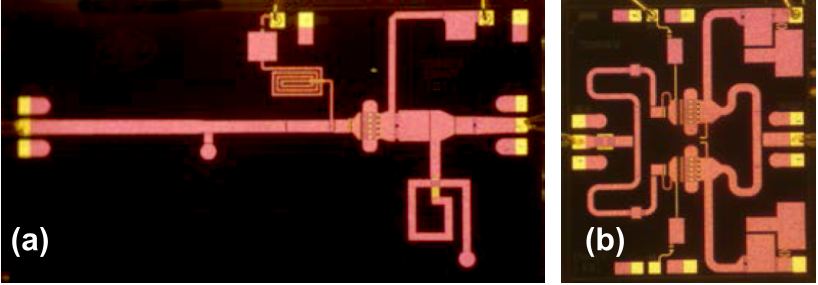
\includegraphics[width=3.45in]{IMS2014_Pictures_PA.png}
\caption{ X-Band MMIC power amplifiers used as rectifiers : (a) Circuit-A: Single stage, $10\times100\mu m$. $3.8\times2.3mm^2$ and (b) Circuit-B: Single stage, two $10\times100\mu m$. $2.0\times2.3mm^2$.}
\label{picture}
\end{figure}


% ==========================
% # III. Measurement Setup #
% ==========================

\section{Measurement Setup}
The measurement setup is based on the SWAP X-402 \cite{Verspecht2010,Roblin2011}. This 4 channels time-domain receiver, working like a LSNA \cite{Verspecht2005} thanks to bi-directional couplers, acquires absolutes incident and reflected waves at DUT's inputs and output ports. Thanks to a relative SOLT and a power calibration, the setup provides time domain RF waveforms for voltages and currents at the calibration reference planes. The SWAP enables measurements in a $30$ GHz RF bandwidth : only the fundamental and the second harmonic were measured. Nevertheless, this paper focus only on the fundamental RF frequency.

During power amplifier measurements, the RF signal is injected at the input of the DUT (gate's port). The DC-to-RF efficiency is calculated according the the output power, the input power and the bias consumption in term of Power Added Efficiency ($\eta_{PA}$) or Drain Efficiency ($\eta_{DE}$) such as :
\begin{eqnarray}
\eta_{PA}=\frac{P_{out}\left(f_0\right)-P_{in}\left(f_0\right)}{P_{DC}} \; ; \; \eta_{DE}=\frac{P_{out}\left(f_0\right)}{P_{DC}}
\end{eqnarray}
Power amplifier characterization where performed with a $50\,\Omega$ RF load applied to the drain RF port.

\begin{figure}[ht!] %!t
\centering
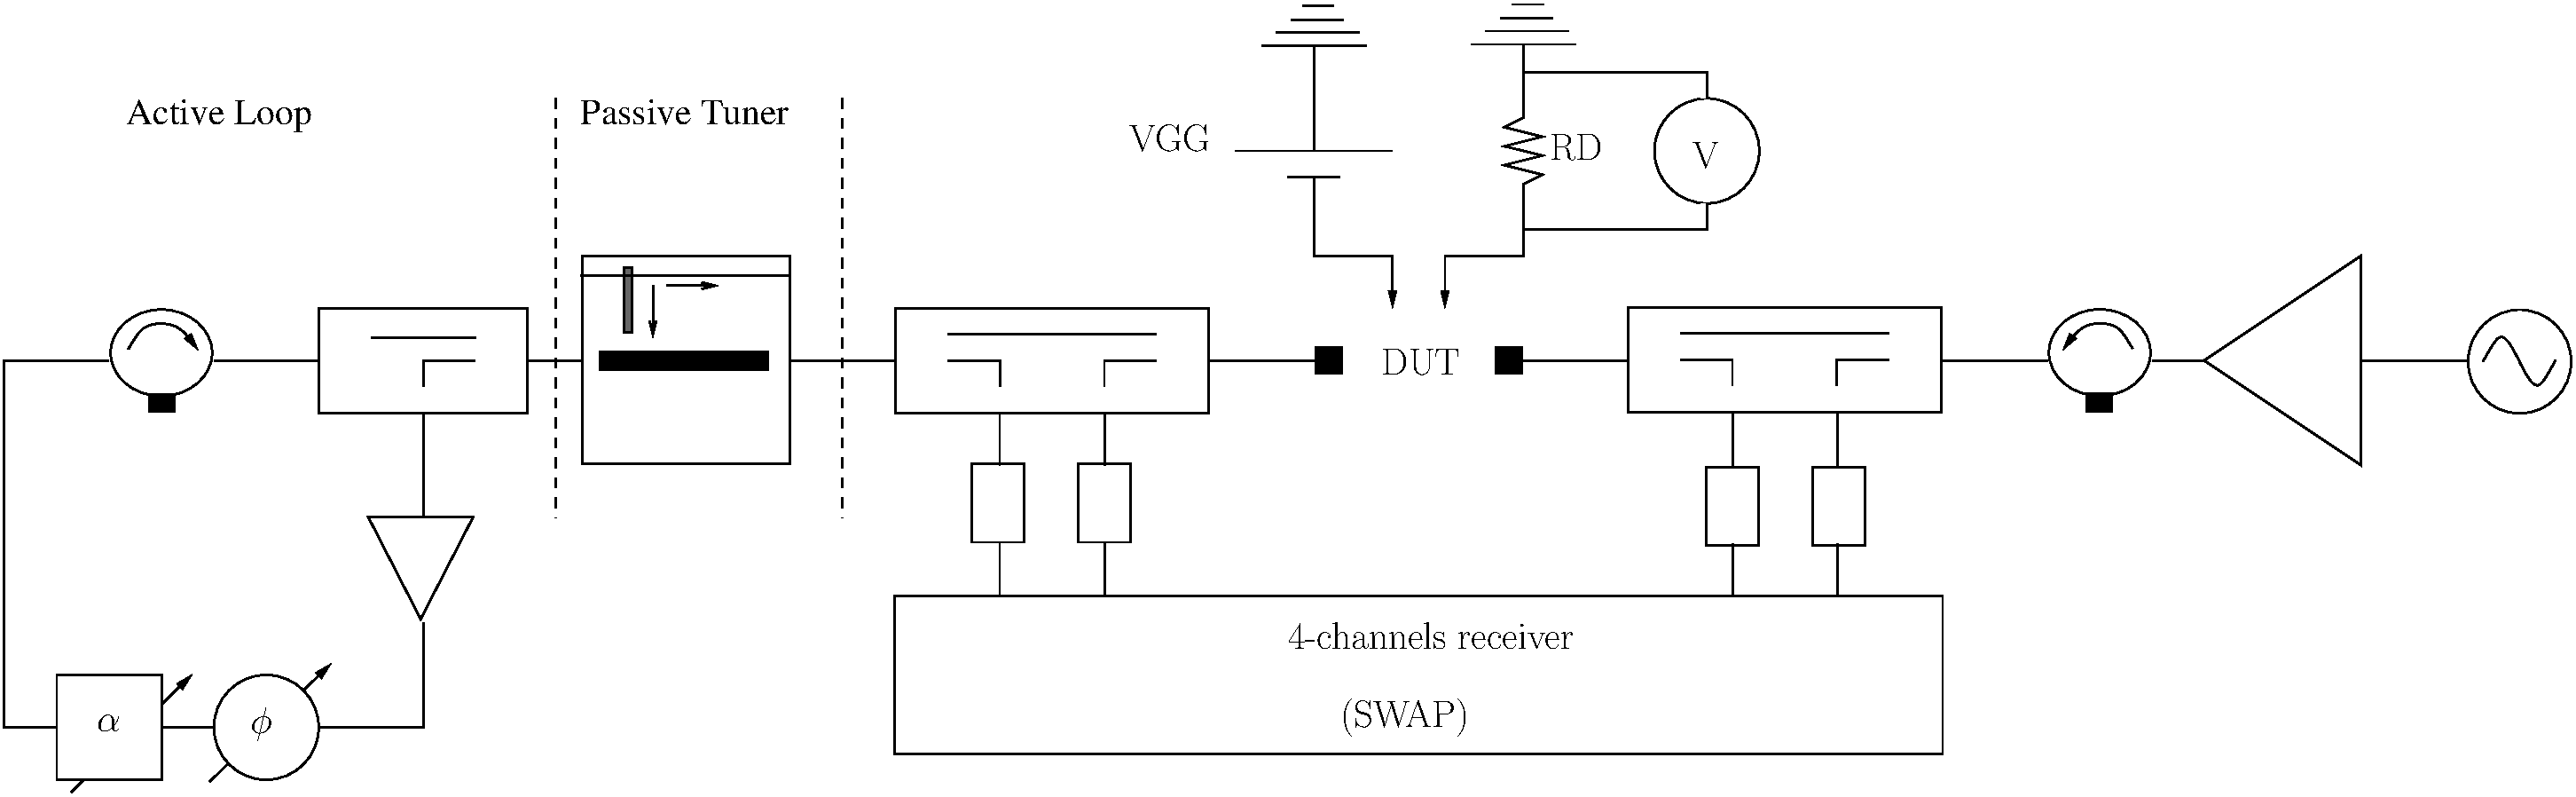
\includegraphics[width=3.4in]{IMS2014_bench.pdf}
\caption{ Time-domain measurement setup for rectifier characterizations. A load-pull is applied on the gate RF port of the DUT. It as been perform with a passive tuner and an active loop for highly reflective load impedance at 10.1 GHz.}
\label{bench}
\end{figure}

Regarding the rectifier characterizations, the RF signal is injected at the RF drain port of the DUT. The output of the rectifier is the DC path of the drain port. The PA is only biased on the gate. In order to obtain the best efficiency, DC-load on the drain (RD) and RF load on the gate are tuned as depicted on Fig. \ref{bench}. The load-pull is performed at the fundamental frequency (10.1 GHz) with a passive tuner. High magnitude on reflexion coefficients have been reached with an active loop.
The RF-to-DC or rectifier efficiency is given by :
\begin{eqnarray}
\eta_{R}=\frac{P_{DC}}{P_{RF\,injected}}=\frac{2{\left|V_{DC}\right|}^2}{RD \times \Re{\left\{V_{drain}\left(f_0\right)I^{*}_{drain}\left(f_0\right)\right\}}}
\end{eqnarray}
Power amplifiers have been measured in a coaxial test-fixture. The error-boxes of the test-fixture have been extracted thanks to a TRL calkit. Performances given is this paper are de-embedded to the input and output GSG ports pictured on Fig.\;\ref{picture}.


% ========================
% # IV. Measured Results #
% ========================

\section{Measured Results}

% ================== Circuit A ==================
\subsection{Circuit-A: one $10\times100\mu m$}
Circuit-A, working as an amplifier, loaded with $50\,\Omega$ and measured at $f_0=10.1\,GHz$, exibits, as shown in Fig. \ref{mike_amp}, its best efficiency $\eta_{PA}=67.87\%$ and $\eta_{DE}=78.36\%$ with $P_{in}=26.42\,dBm$ and  $P_{out}=35.16\,dBm$. The best bias point for efficiency is VGG=-4.0V and VDD=20V. The design is optimized for a bias point close to class-B.

\begin{figure}[ht!] %!t
\centering
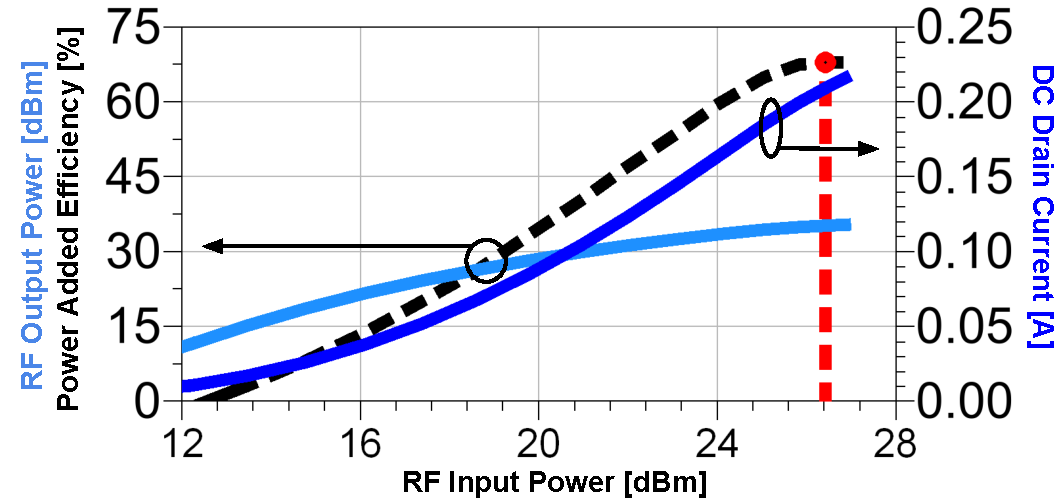
\includegraphics[width=2.5in]{IMS2014_Mike_Amplifier.pdf}
\caption{ Circuit-A best efficiency performances as an amplifier are measured with $VGG=-4.0\,V$ and $VDD=20\,V$. Light blue curve is the output power, dark blue is the DC current on the drain and the efficiency ($\eta_{PA}$) is traced with a black dashed line. The maximum efficiency is $\eta_{PA}=67.87\%$ at $P_{in}=26.42\,dBm$ (red dashed line).}
\label{mike_amp}
\end{figure}

This circuit has been characterized as a rectifier with the bench depicted on Fig. \ref{bench}. In order to optimize the RF-to-DC efficiency ($\eta_R$), we can adjust 3 parameters : the gate bias voltage ($VGG$), the DC load impedance at the output ($RD$) and the RF load impedance on the gate ($Z_{load}$ or $\Gamma_{load}$). \\

\begin{itemize}
	\item {$Z_{load}$ is a prime of importance regarding the rectifying efficiency of the circuit as illustrated for S-band in \cite{Reveyrand2012}.\\}
		
	\item {$VGG$ should correspond to a class-B or class-C to be compliant with the rectifier effect on a transistor. $VGG$ has a moderate influence on the efficiency compared to $Z_{load}$. In this work, we noticed a deep class-C bias point make possible to reach the best rectifying efficiency. Fig. \ref{mike_rect_mVGG} illustrates a VGG sweep for fixed $Z_{load}$ and $RD$. $\eta_R=60.37\%$ has been measured at $P_{RF}=34.63\,dBm$ but $Z_{load}$ is not optimized (limited by the passive tuner during our automated multi-sweep measurements).}

\begin{figure}[ht!] %!t
\centering
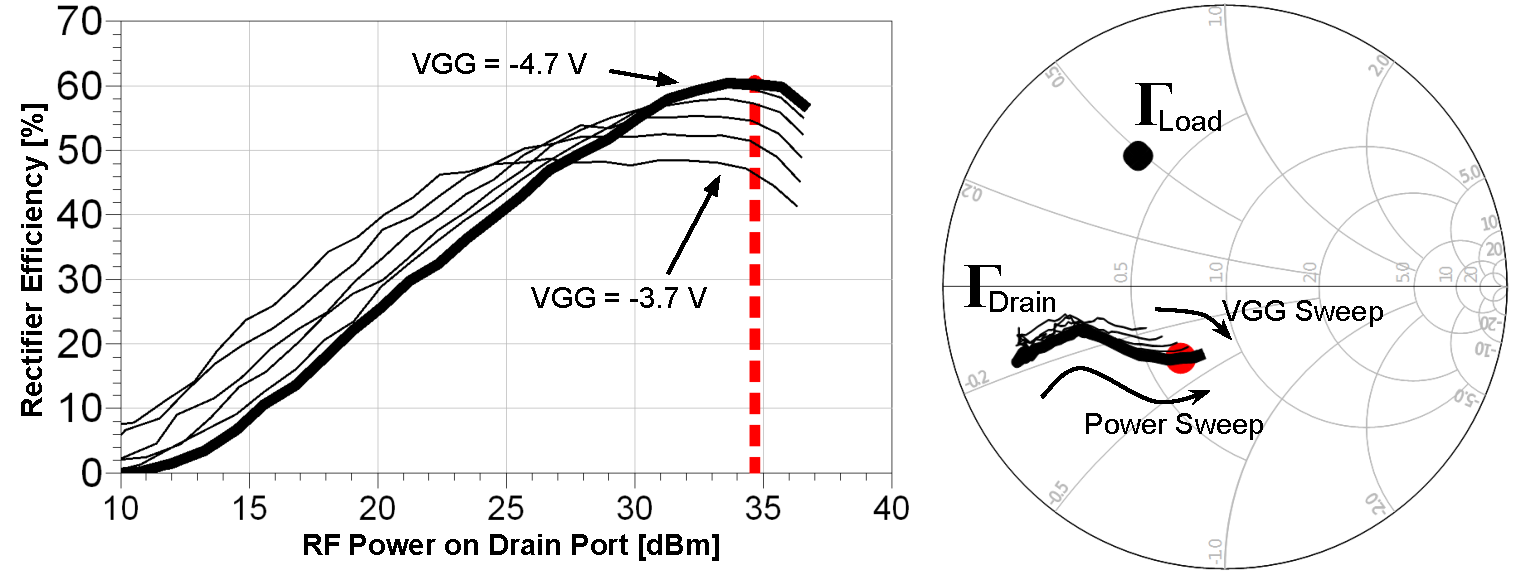
\includegraphics[width=3.4in]{IMS2014_Mike_Rectifier_mVGG.pdf}
%\epsfxsize=3.25in\epsfbox{figure1.epsi}
\caption{ Circuit-A rectifying performances for several $VGG$ (from $-3.7\,V$ to $-4.7\,V$ with a $0.2\,V$ step). The gate's RF port is loaded at fundamental frequency, with $Z_{load}=(17.9+j\,24.0)\Omega$ and the drain DC load impedance is $RD=100\Omega$.}
\label{mike_rect_mVGG}
\end{figure}

	\item {$RD$ range should be limited by the DC voltage and current values the transistor can handle. This value will establish the DC output power distribution between voltage and current. This parameters impacts the RF impedance at the input of the rectifier (drain's RF port) but has a limited influence on the maximum measured efficiency.}
\end{itemize}
Influences of those 3 parameters are summerized in table \ref{tab:var}.

After optimization of $Z_{load}$, $RD$ and $VGG$ on circuit-A, the best rectifying efficiency $\eta_R=64.40\%$ is obtained at $VGG=-4.7\,V$, $RD=100\Omega$ and  $Z_{load}=(8.45+j\,24.5)\Omega$. The RF power sweep results are depicted on Fig. \ref{mike_rect}. $Z_{load}$ has been applied thanks to the active loop. The RF power measured at the gate's port reference plane is displayed too and demonstrates the fact that the PA can work as an efficient self-synchroneous rectifier thanks to a passive load applied to the gate's RF port.

\begin{figure}[ht!] %!t
\centering
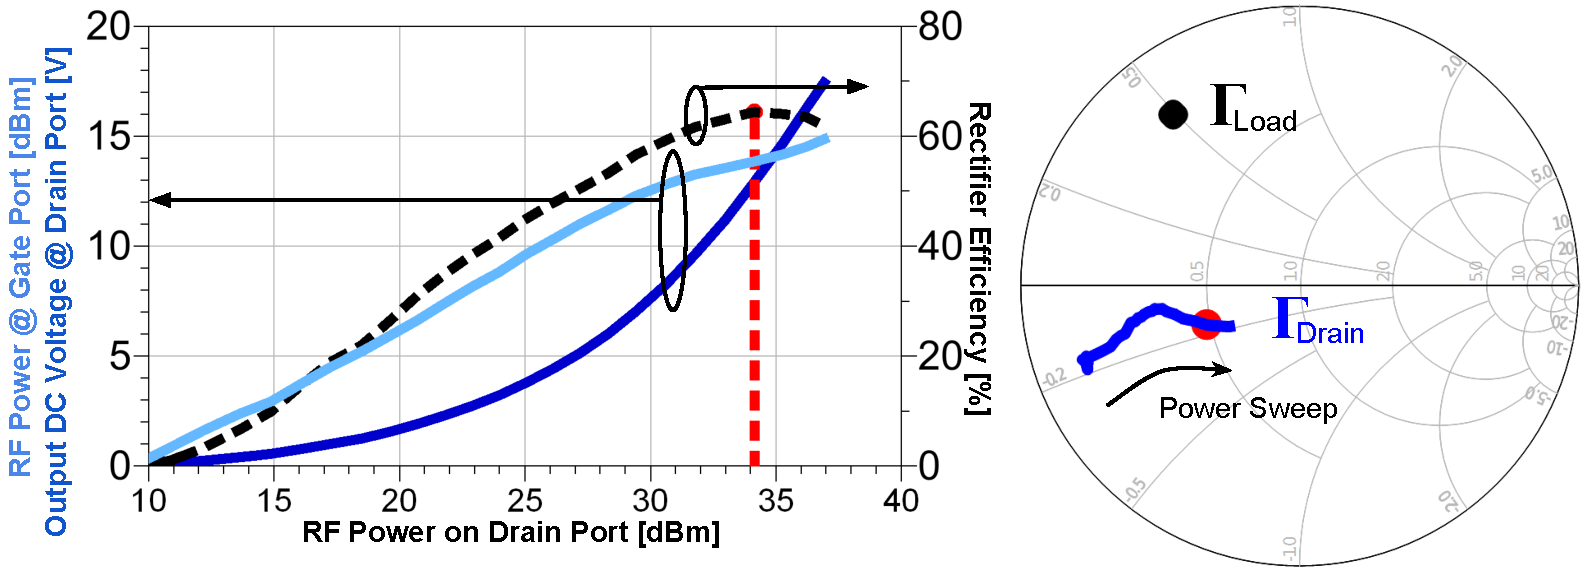
\includegraphics[width=3.4in]{IMS2014_Mike_Rectifier.pdf}
\caption{ Circuit-A :  Rectifier efficiency $\eta_R$ (black dashed line), DC output drain voltage (dark blue) and RF power at the gate reference plane (light blue) versus Injected drain RF power. The best rectifying performance is $\eta_R=64.4\%$ at $P_{RF}=34.14\,dBm$ (red dashed line). The smith chart on the right shows the optmal load impedance presented at the gate port (black dot) and the drain impedance of the DUT (blue curve) during the power sweep.
}
\label{mike_rect}
\end{figure}

\begin{table}[ht]
\caption{Impact on rectifier efficiency and drain RF impedance} %title of the table
\centering
\begin{tabular}{|c| c | c |  }
\hline
 &Efficiency & RF drain impedance\\
\hline
$Z_{load}$ & High & Medium\\
$RDD$ & Low & High\\
$VGG$ & Medium & Low\\
\hline
\end{tabular}
\label{tab:var}
\end{table}


% ================== Circuit B ==================

\subsection{Circuit-B: two $10\times100\mu m$}
Circuit-B has been characterized in the same manner than circuit-A for both amplifier and rectifier modes.
Regarding the amplifier measurements, with a $50\,\Omega$ load, at $10.1\,GHz$, circuit B exhibits the best efficiency $\eta_{PA}=56.47\%$ and $\eta_{DE}=65.75\%$ with $P_{in}=26\,dBm$ and  $P_{out}=35\,dBm$. The bias point is VGG=-3.4V and VDD=20V.
The design of the amplifier is optimized for deep class-AB.

\begin{figure}[ht!] %!t
\centering
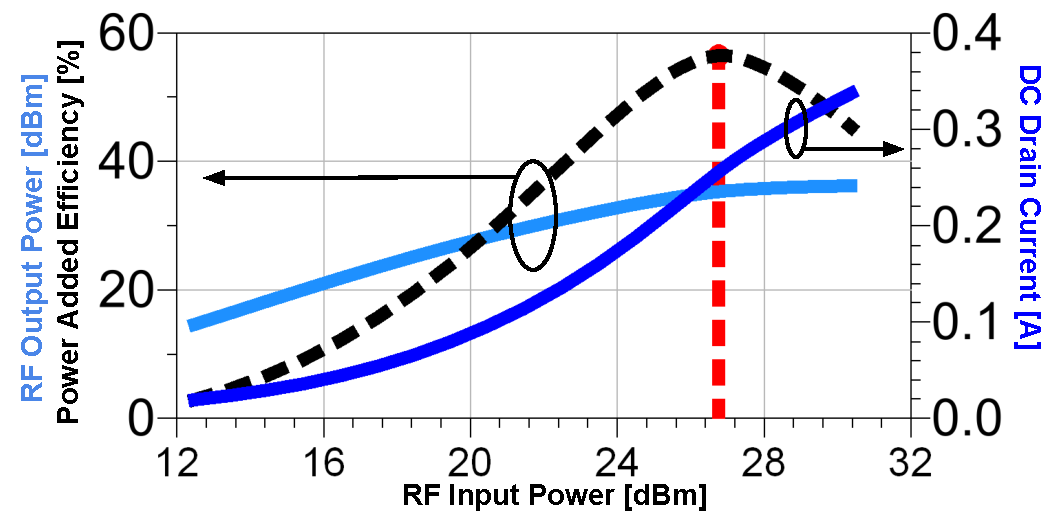
\includegraphics[width=2.5in]{IMS2014_Scott_Amplifier.pdf}
\caption{ Circuit-B as an amplifier:  PAE $\eta_{PA}$ (black dashed line), Output RF power (light blue) and DC drain current (dark blue) versus input RF power. The best efficiency is $\eta_{PA}=56.47\%$ at $P_{in}=26\,dBm$ (red dashed line) with $VGG=-3.4\,V$, $VDD=20\,V$.
 }
\label{scott_amp}
\end{figure}

Rectifier measurements were performed on circuit-B. After an optimization on the variables $Z_{load}$, $RD$ and $VGG$. This HEMT-PA-based rectifier is $63.94\%$ efficient. Once again, $Z_{load}$ has been reach thanks to the active loop depicted on Fig. \ref{bench}. The measured RF power sweep is shown in Fig. \ref{scott_rect}. As shown with Circuit-A, we can notice the RF power located at the gate port (light blue line) making possible the use of a passive impedance to reach a good rectifying efficiency.

\begin{figure}[ht!] %!t
\centering
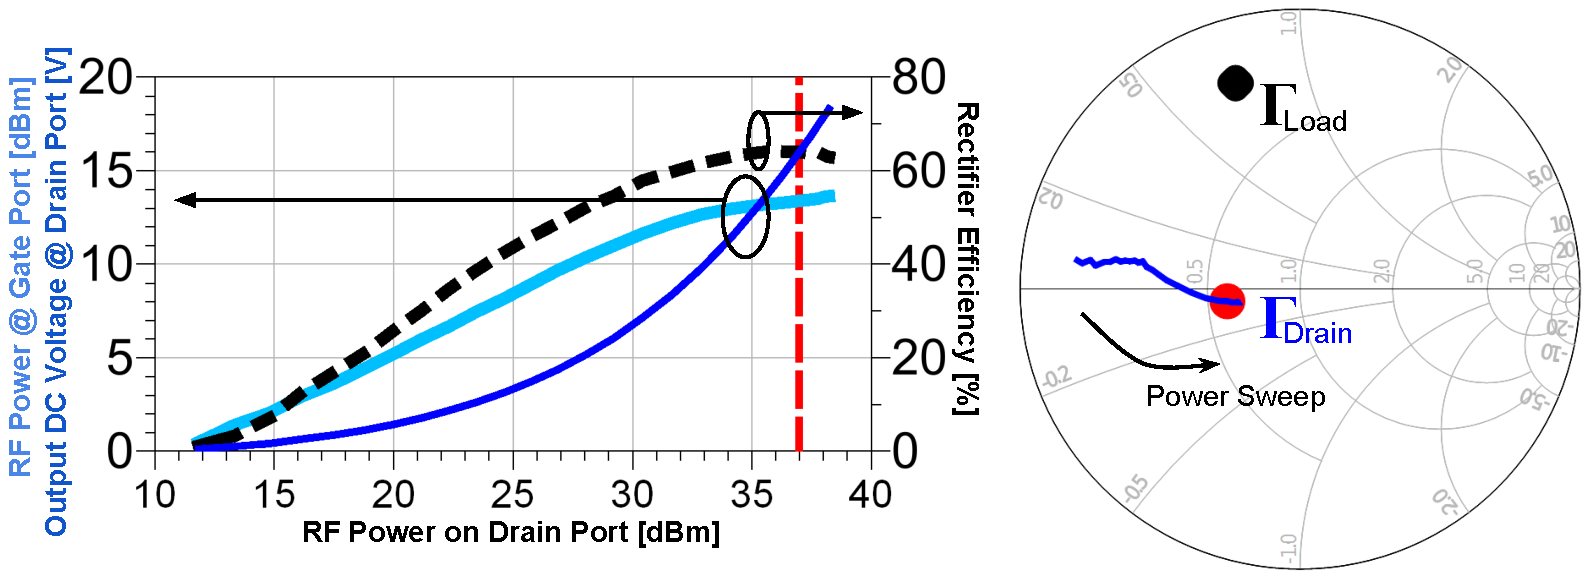
\includegraphics[width=3.4in]{IMS2014_Scott_Rectifier.pdf}
\caption{ Circuit-B best rectifying performances with $VGG=-4.7V$, $RD=80\,\Omega$ and a RF impedance load applied on the gate port $Z_{load}=(9.8 + j\,35.75)\,\Omega$. The circuit exhibit a rectifying efficiency $\eta_R=63.94\%$ with 37dBm RF power injected on the drain port. RF power  at the gate port (light blue), output DC voltage (dark blue) and rectifying efficiency (black dash) are display on the left chart. Right chart display the rectifier's input impedance $\Gamma_{Drain}$ (drain port) and load impedance $\Gamma_{Load}$ (gate port).
 }
\label{scott_rect}
\end{figure}

Finally, table \ref{tab:hresult} summaries performances of the two X-Band GaN MMICs for both amplifier and rectifier operation modes. In the case of amplifier mode, $\eta_{PA}$ is the displayed \textit{efficiency}. The \textit{RF power} is the power located at the drain RF port.
By presenting good efficiency even at X-Band, this work highlights the possibility to use HEMT GaN for designing a rectifying element. Therefore, there is a need for nonlinear models working both for amplification and rectification. Intrinsic nonlinear capacitances, for example, may  be extracted from first and third quadrants.

\begin{table}[ht]
\caption{Performances as amplifier and rectifier at 10.1 GHz} %title of the table
\centering % centering table
\begin{tabular}{c| rr | rr  } % creating eight columns
\hline\hline %inserting double-line
 &\multicolumn{2}{c}{Amplifier} & \multicolumn{2}{c}{Rectifier}\\
Circuit &A&B&A&B\\ [0.25ex]
\hline
Max Efficiency(\%) & 67.87 & 56.47 & 64.40 & 63.94 \\
DC Power (mW) & 4186 & 5112 & 1671 & 3182\\
 RF Power (mW) & 3281 & 3362 & 2594 & 4976\\
\hline\hline
\end{tabular}
\label{tab:hresult}
\end{table}


% ==================
% # Conclusion #
% ==================
\section{Conclusion}
This work shows measured results on two X-Band GaN MMIC ($0.15\,\mu m$ process). High efficiencies (higher than $56\%$) are obtained for both amplification and rectification modes. Rectification is performed in self-synchroneous way without any injection on the gate RF port. A passive termination is self-sufficient at microwave frequencies thanks to the Miller effect produced by $C_{gd}$ in the HEMT GaN intrinsic non-linear model.


% ==================
% # Acknowledgment #
% ==================
% use section* for acknowledgment
%\section*{Acknowledgment}
%For the Summary paper submission only, no %acknowledgements are allowed.


% ==============
% # REFERENCES #
% ==============
\begin{thebibliography}{1}

\bibitem{TrustZone} 
\emph{ARM Security Technology: Building a Secure System using TrustZone Technology}, 2009. Ref. no. PRD29-GENC-009492C.

\bibitem{SGX}F. McKeen, I. Alexandrovich, A. Berenzon, C. V. Rozas, H. Shafi, V. Shanbhogue, and U. R. Savagaonkar.
\emph{Innovative instructions and software model for isolated execution. In Hardware and Architectural
Support for Security and Privacy �C HASP, ACM, page 10}, 2013. 

\bibitem{TIMBERV}S. Weiser, M. Werner, F. Brasser, M. Malenko, S. Mangard and A. Sadeghi.
\emph{TIMBER-V: Tag-Isolated Memory Bringing Fine-grained Enclaves to RISC-V},
Proc. NDSS, 2019.

\bibitem{HDFI}C. Song, H. Moon, M. Alam, I. Yun, B. Lee, T. Kim, W. Lee, and Y. Paek. 
\emph{HDFI: Hardware-Assisted Data-Flow Isolation},
In Security and Privacy 16, pages 1�C17. IEEE Computer Society, 2016.

\bibitem{RISCV}A. Waterman and K. Asanovic. 
\emph{The risc-v instruction set manual,
volume i: User-level isa, version 2.2. Technical report, SiFive Inc},
EECS Department, University of California, Berkeley, 2017.

\end{thebibliography}

\end{document}
